\documentclass[a4paper,12pt]{article}
\usepackage{a4wide}
\usepackage{tikz}
\usetikzlibrary{calc}
\usepackage{hyperref}
\usepackage{color}
\usepackage{pdflscape}
\usepackage{bytefield}
\usepackage{rotating}
\usepackage{caption}

\newlength{\maxheight}
\setlength{\maxheight}{\heightof{W}}
\newcommand{\baselinealign}[1]{
	\centering
	\raisebox{0pt}[\maxheight][0pt]{ #1 }
}

\newcommand{\bitlabel}[2]{
	\bitbox[]{ #1 }{
		\raisebox{0pt}[4ex][0pt]{
			\turnbox{45}{\fontsize{7}{7}\selectfont#2}
		}
	}
}

\begin{document}
\pagestyle{empty}
\setlength{\parindent}{0em}
\section*{Register File}

Your task is to program the behavior of an entity called ``register\_\,file". This entity is declared in the attached file ``register\_\,file.vhdl" and has the following properties:
\begin{itemize}
\item Input:  IN1 with type std\_logic\_vector  of length {{n}}
\item Input:  WA1 and RA with type std\_logic\_vector of length {{address_width_n}}

\item Input:  WA2 with type std\_logic\_vector of length {{address_width_reg0}}


\item Input:  WE1, WE2 and IN2 with type std\_logic

\item Input:  CLK with type std\_logic


\item Output: Output with type std\_logic\_vector of length {{n}}
\end{itemize}

\begin{center}
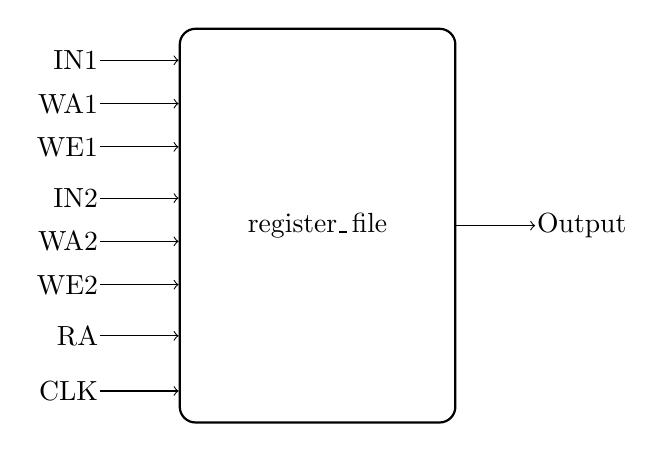
\begin{tikzpicture}
\draw node [draw,rectangle, minimum height=50mm, minimum width=35mm,rounded corners=2mm,thick](entity){};

\draw[->] ($ (entity.west)+(-10mm,21mm)$) -- ($ (entity.west) + (0mm,21mm)$);
\draw[anchor=east] node at ($ (entity.west)+(-9mm,21mm)$){IN1};

\draw[->] ($ (entity.west)+(-10mm,15.5mm)$) -- ($ (entity.west) + (0mm,15.5mm)$);
\draw[anchor=east] node at ($ (entity.west)+(-9mm,15.5mm)$){WA1};

\draw[->] ($ (entity.west)+(-10mm,10mm)$) -- ($ (entity.west) + (0mm,10mm)$);
\draw[anchor=east] node at ($ (entity.west)+(-9mm,10mm)$){WE1};


\draw[->] ($ (entity.west)+(-10mm,3.5mm)$)  -- ($ (entity.west) + (0mm,3.5mm)$);
\draw[anchor=east] node at ($ (entity.west)+(-9mm,3.5mm)$){IN2};

\draw[->] ($ (entity.west)+(-10mm,-2mm)$)  -- ($ (entity.west) + (0mm,-2mm)$);
\draw[anchor=east] node at ($ (entity.west)+(-9mm,-2mm)$){WA2};

\draw[->] ($ (entity.west)+(-10mm,-7.5mm)$) -- ($ (entity.west) + (0mm,-7.5mm)$);
\draw[anchor=east] node at ($ (entity.west)+(-9mm,-7.5mm)$){WE2};


\draw[->] ($ (entity.west)+(-10mm,-14mm)$) -- ($ (entity.west) + (0mm,-14mm)$);
\draw[anchor=east] node at ($ (entity.west)+(-9mm,-14mm)$){RA};


\draw[->] ($ (entity.west)+(-10mm,-21mm)$) -- ($(entity.west) + (0mm,-21mm)$);
\draw[anchor=east] node at ($ (entity.west)+(-9mm,-21mm)$){CLK};



\draw[->] ($ (entity.east) + (0mm,0mm)$) -- ($ (entity.east) + (10mm,0mm)$);
\draw[anchor=west] node at ($ (entity.east) + (9mm,0mm)$){Output};

\draw node at ($ (entity) - (0,0mm)$){register\_\,file};

\end{tikzpicture}
\end{center}

Do not change the file ``register\_\,file.vhdl".\\

The ``register\_\,file" entity shall contain {{N_n}} registers which have to be {{n}} bit wide each. The input data for registers 1 to {{N_n_minus_1}} comes from the input IN1 and is written to the register specified by the write address WA1 only if the write enable bit WE1 is set to `1'. The write address WA2 is used to access the {{lower}} {{special_reg0_size}} bits of the register 0 seperately.
The input data for the register 0 comes from the input IN2 and shall only be written if the write enable bit WE2 is `1'.
The output of the entity is the content of a register selected by the read address RA.
See Figure~1 for a structural representation of this register file. \\

Changes of input signals shall become effective at a rising edge of the input CLK signal.\\

{{bypass_or_read_priority_text1}} {{bypass_or_read_priority_text2}}

\begin{figure}[h!]
	\centering
	\captionsetup{justification=centering,margin=1cm}
	\begin{bytefield}[rightcurly=., rightcurlyspace=0pt, boxformatting=\baselinealign]{ {{n}} }
		{{bitlabel}} \\
		\bitheader[endianness=big]{ {{reg0_bitheader_bits}} {{n_minus_1}}  } \\

		\begin{rightwordgroup}{00h}
		\begin{leftwordgroup}{Register 0}
			\bitbox{ {{n_minus_reg0_size}} }{} {{bitbox}}
		\end{leftwordgroup}
		\end{rightwordgroup} \\

		\begin{rightwordgroup}{01h}
			\bitbox{ {{n}} }{Register 1}
		\end{rightwordgroup} \\

		{{dots_or_bitbox}}

		\begin{rightwordgroup}{0{{N_n_minus_2}}{}h}
			\bitbox{ {{n}} }{Register {{N_n_minus_2}} {}}
		\end{rightwordgroup} \\

		\begin{rightwordgroup}{0{{N_n_minus_1}}{}h}
			\bitbox{ {{n}} }{Register {{N_n_minus_1}} {}}
		\end{rightwordgroup} \\

	\end{bytefield}
	\caption{The layout of the register file. Addresses are given as a hexadecimal representation of the binary value.}
\end{figure}


This behavior, described above, has to be programmed in the attached file ``register\_\,file\_beh.vhdl".\\



To turn in your solution write an email to {{SUBMISSIONEMAIL}} with Subject ``Result Task {{TASKNR}}" and attach your file ``register\_\,file\_beh.vhdl".

\vspace{0.7cm}
Good Luck and May the Force be with you.


\end{document}
